\documentclass[11pt,letterpaper]{article}
\usepackage[utf8]{inputenc}
\usepackage{hyperref}



%----- Configuración del estilo del documento------%
\usepackage{epsfig,graphicx}
%% Ruta de las imágenes
\graphicspath{{resources/}}
\usepackage{geometry}
\usepackage{fancyhdr}
\usepackage{lastpage}
\pagestyle{fancy}
\usepackage{float}
\fancyhf{}

% Encabezado
\fancyhead[L]{\textit{Práctica 4: Cifrados Clásicos}}

% Pie de página
\fancyfoot[L]{\textit{Facultad de Ciencias, 2025-I}}
\fancyfoot[R]{\textit{Criptografía y Seguridad}}

%-------------------------------------------------%


%%Para la bibliografía
\usepackage[style=apa, backend=biber]{biblatex}
\addbibresource{referencias.bib}



\begin{document}

\newgeometry{left=2cm,right=2cm,top=1.8cm,bottom=2.3cm} % Cambiar los márgenes solo para la primera página

\begin{titlepage}
    \begin{center}
        \rule{17cm}{0.1mm}
    \end{center}
    \begin{center}
        \begin{minipage}{3cm}
            \begin{center}
                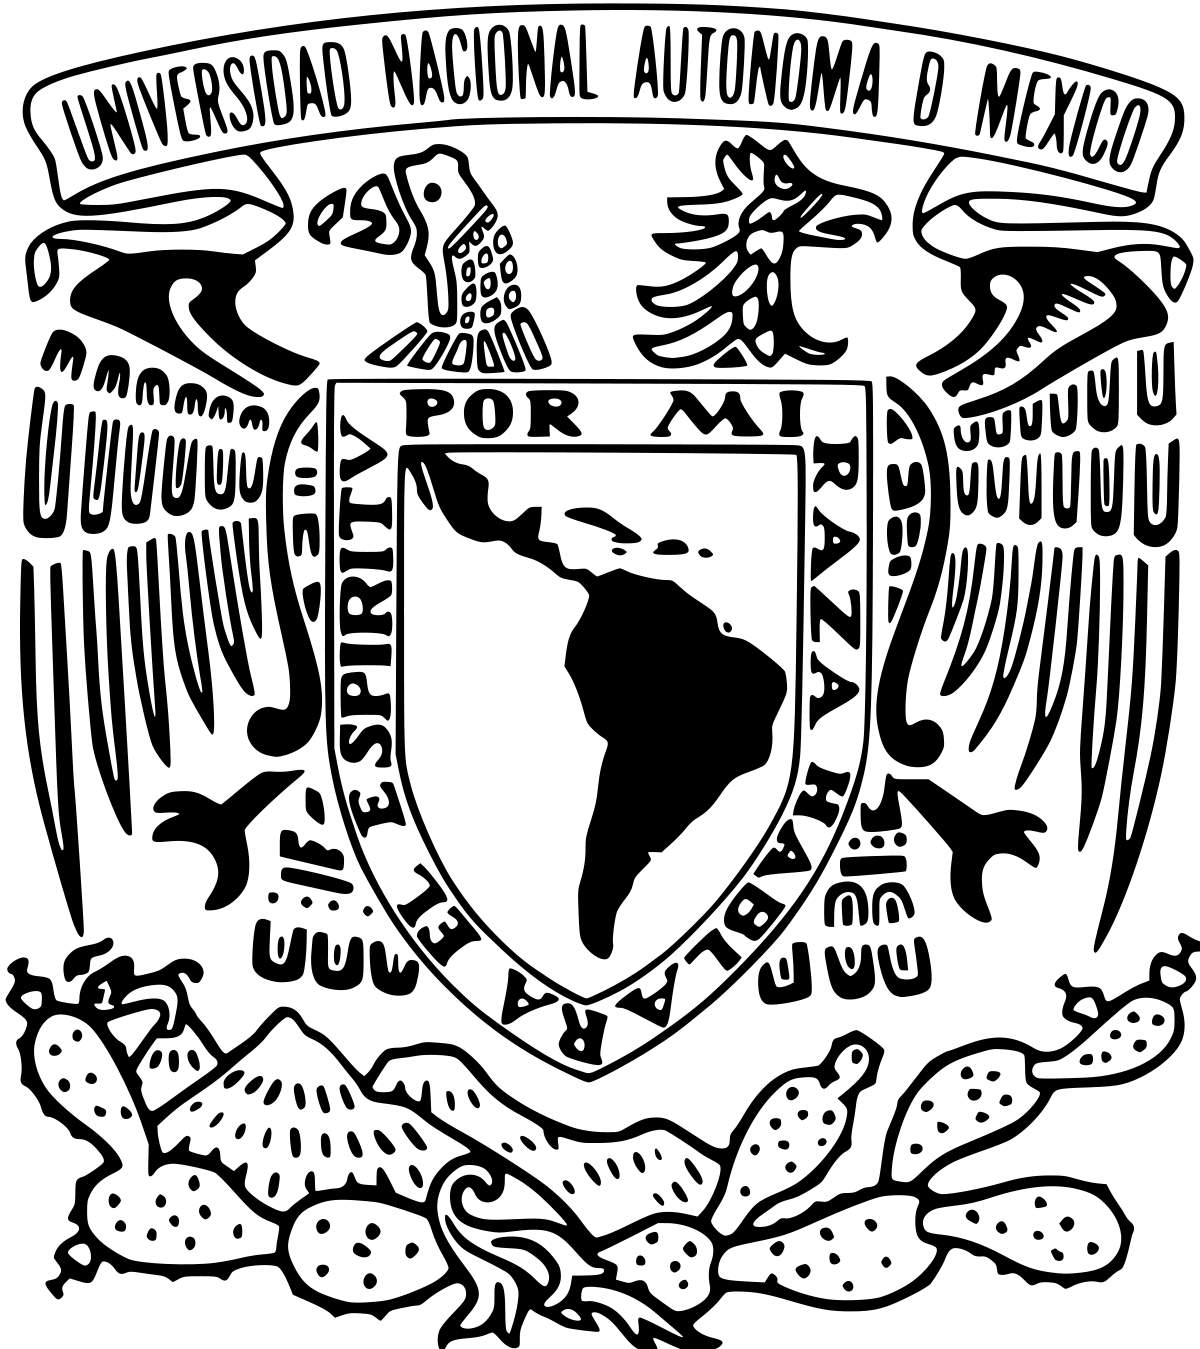
\includegraphics[height=3.4cm]{Logo_UNAM.png}
            \end{center}
        \end{minipage}\hfill
        \begin{minipage}{10cm}
    
            \begin{center}
                \large
                \textbf{ Universidad Nacional Autónoma de México}\\[0.1cm]
                \textbf{Facultad de Ciencias}\\[0.1cm]
                \textbf{Criptografía y Seguridad}\\[0.1cm]
                \textbf{Semestre 2025-1}\\[0.1cm]
            \end{center}
        \end{minipage}\hfill
        \begin{minipage}{3cm}
            \begin{center}
                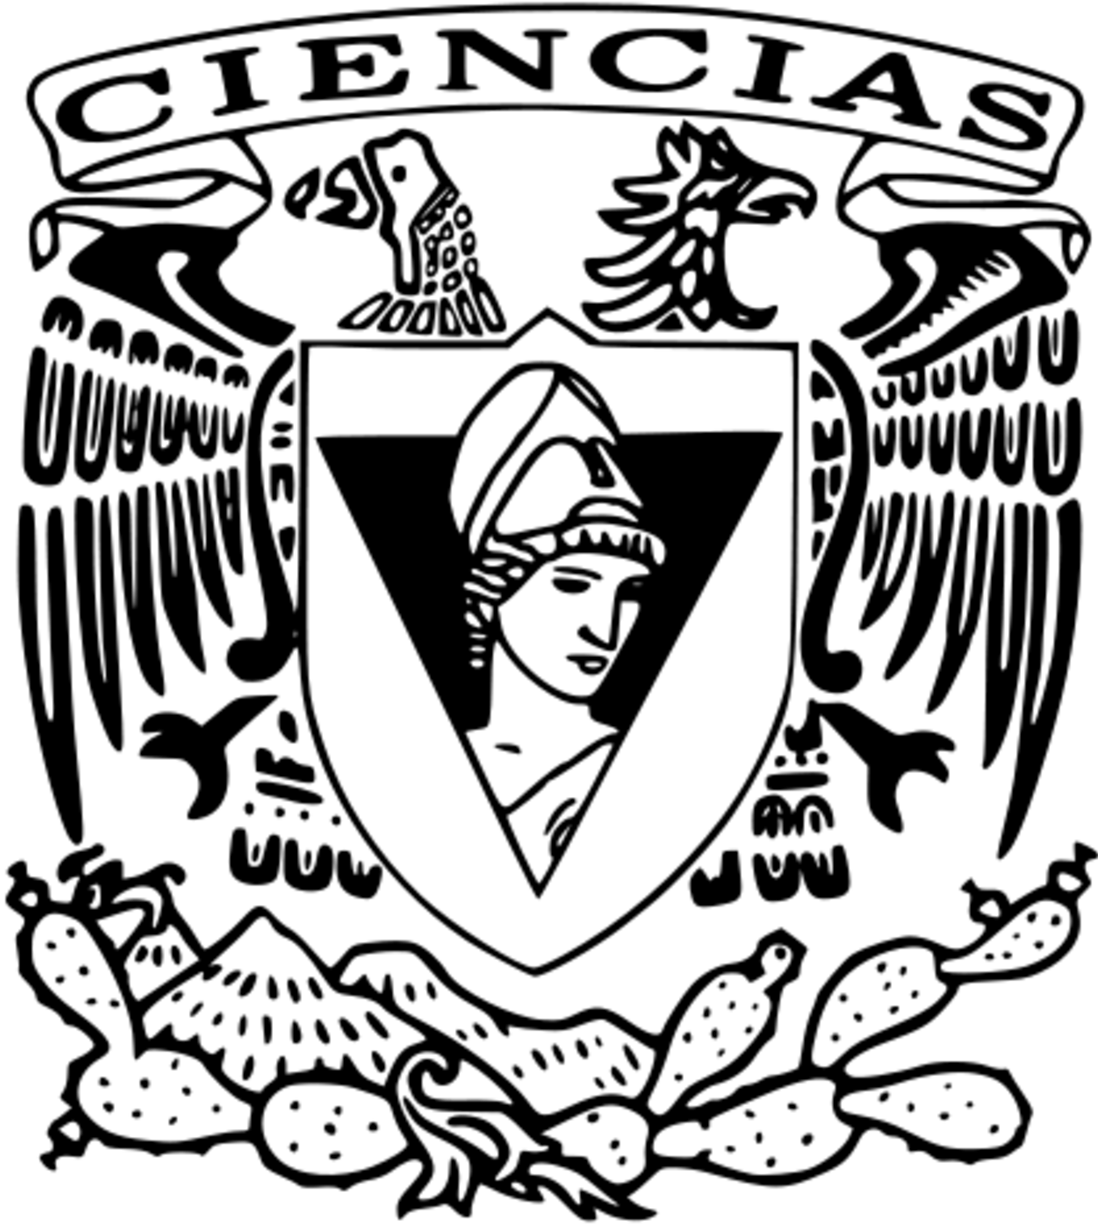
\includegraphics[height=3.4cm]{Logo_FC.png}
            \end{center}
        \end{minipage}
    \end{center}

    \vspace{2cm}
    
    \begin{center}
        {\Huge Práctica 4: Cifrados Clásicos}
    \end{center}
    
    \vspace{2cm}
    
    \begin{center}
        \large

        \textsc{Equipo: \\
                \textbf{Barrientos Sánchez José Antonio\\
                Hernandez Gonzalez Yun\\
                Ortiz Castañeda José Ramón}}\\[0.5cm]     
                
                \textsc{{Fecha de entrega: \\ \textbf{10 de septiembre de 2024}}}\\[0.5cm]        

                \textsc{{Profesor: \\ \textbf{ Anayanzi Delia Martínez Hernández}}}\\[0.5cm]  

                \textsc{Ayudantes: \\\textbf{Cecilia del Carmen Villatoro Ramos \\
                José Angel Arévalo Avalos \\
                Ivan Daniel Galindo Perez \\
                David Armando Silva de Paz}}
    \end{center}
    
    \vfill
    
    \begin{center}
        \rule{17cm}{0.1mm}
    \end{center}
    
\end{titlepage}

\restoregeometry % Restaurar los márgenes originales

\tableofcontents

\section{Introducción}




\section{Desarrollo.}


\section{Preguntas.}
\begin{enumerate}
\item ¿Cuántos primos relativos hay en $Z_{256}$?
Primero, vamos a descomponer en factores primos a 256:
  $$ 256 = 2^8$$
Con la fórmula del totiente de Euler podemos saber el númerp de primos relativos:
 $$\phi(256) = 256 \times \frac{1}{2} = 128$$
Por lo tanto, el número de primos relativos en $ Z_{256} $ es $ \phi(256) = 128 $.
\item pregunta2
\item ¿Cuántas posibles combinaciones no triviales existen para cifrar bytes con César, Decimado
y Afin?
\begin{itemize}
\item \textbf{Cifrado Cesar}

Primero debemos notar que los bytes tienen 256 valores.
Para el \textbf{Cifrado César},  sabemos funciona con un desplazamiento, en el que cada byte se reemplaza con $(x + k) mod 256$ donde k es la llave del desplazamiento. Por lo tanto, si se está usando un desplazamiento, solo tenemos tantas combinaciones como valores, por lo que tenemos \textbf{256 combinaciones}.

\item \textbf{Cifrado Decimado}
El cifrado decimado funciona cuando multiplicamos el valor del byte x por un llave k, para después hacer $mod 256$. Entonces, si qieremos invertir esta operación, $k$ debe der ser primo relativo  de 256, y como ya vimos anteriormente, 256 solo tiene 1\textbf{28 primos relativos} 

\item \textbf{Cifrado Afin}
El cifrado afín es una combinación del cifrado César y el cifrado Decimado, el cuál utiliza la siguiente función $(a\cdot x + b) mod 256$ en el que a es una constante primo relativo y b es una constante de desplazamiento.
Así que la combinación de los dos nos da $128 \cdot 255 = 32, 640$
\end{itemize}
\item ¿Por qué el sistema de archivos de UNIX, aunque un archivo tenga una extensión diferente
(o incluso no tenga), sigue reconociendo al archivo original?
Ya que el sistema de archivos en UNIX no usa las extensiones para reconocer archivos, se debe a que UNIX trabaja directamente con el contenido del archivo, utilizando propiedades internas como los \textit{números mágicos} para identificar el tipo de archivo, por lo que permite que los archivos sean reconocidos y gestionados independientemente de su nombre o extensión. \cite{linux}
\item ¿Por qué los archivos descifrados tienen exactamente el mismo tamaño que antes de cifrar,
pero no pudimos leerlos? ¿Por qué no tuvimos que agregar/quitar nada?
Porque el tamaño no es relavante a la hora de cifrar, ya que no se añade o eliminan bytes, solo se modifican con el cifrado.
\item Ya que base64 no es un cifrado, sino codificación, ¿en qué casos podemos usarlo?
\begin{itemize}
\item Incrustación de datos binarios (como imágenes o archivos de sonido) en HTML, CSS, EML y otros documentos de texto.
\item Garantizar la transferencia, el almacenamiento o la salida seguros de datos que puedan no estar respaldados o dañados.
\item Codificación de certificados SSL, archivos adjuntos de correo electrónico y otra información que requiera el escape de caracteres especiales. \cite{base64}
\end{itemize}
\item Supongamos que estuvieras en Hogwarts y tuvieras que utilizar un búho para comunicarte,
¿cuál crees que sería la mejor opción para mandar mensajes seguros a través de la lechuza?

Para este caso, y con ayuda del video, se puede utilizar Three-pass-protocol, el cual un método para enviar mensajes seguros sin necesidad de intercambiar claves secretas. Para ello, suponiendo que somos Harry Potter, y le queremos enviar un mensaje a Hermione.
\begin{enumerate}
\item Primero ciframos el mensaje $M$ con mi clave $ K_{Harry}$ y enviamos el mensaje cifrado $M'$ a Hermione
\item Ahora, Hermione cifra el mensaje cifrado $ M' $ con su clave $ K_{He} $ obteniendo $ M''$ y lo envía de vuelta a nosotros.
\item  Después, desciframos  $ M'' $ con nuestra clave, eliminando el cifrado y enviamos $ M''' $  de vuelta a Hermione.
\item Finalmente, Hermione descifra $M''' $ con su clave $ K_{He} $ y obtiene el mensaje original $ M $.
\end{enumerate}


\end{enumerate}

\section{Conclusiones}





\printbibliography




\end{document}
